% Options for packages loaded elsewhere
\PassOptionsToPackage{unicode}{hyperref}
\PassOptionsToPackage{hyphens}{url}
%
\documentclass[
]{article}
\usepackage{amsmath,amssymb}
\usepackage{iftex}
\ifPDFTeX
  \usepackage[T1]{fontenc}
  \usepackage[utf8]{inputenc}
  \usepackage{textcomp} % provide euro and other symbols
\else % if luatex or xetex
  \usepackage{unicode-math} % this also loads fontspec
  \defaultfontfeatures{Scale=MatchLowercase}
  \defaultfontfeatures[\rmfamily]{Ligatures=TeX,Scale=1}
\fi
\usepackage{lmodern}
\ifPDFTeX\else
  % xetex/luatex font selection
\fi
% Use upquote if available, for straight quotes in verbatim environments
\IfFileExists{upquote.sty}{\usepackage{upquote}}{}
\IfFileExists{microtype.sty}{% use microtype if available
  \usepackage[]{microtype}
  \UseMicrotypeSet[protrusion]{basicmath} % disable protrusion for tt fonts
}{}
\makeatletter
\@ifundefined{KOMAClassName}{% if non-KOMA class
  \IfFileExists{parskip.sty}{%
    \usepackage{parskip}
  }{% else
    \setlength{\parindent}{0pt}
    \setlength{\parskip}{6pt plus 2pt minus 1pt}}
}{% if KOMA class
  \KOMAoptions{parskip=half}}
\makeatother
\usepackage{xcolor}
\usepackage[margin=1in]{geometry}
\usepackage{longtable,booktabs,array}
\usepackage{calc} % for calculating minipage widths
% Correct order of tables after \paragraph or \subparagraph
\usepackage{etoolbox}
\makeatletter
\patchcmd\longtable{\par}{\if@noskipsec\mbox{}\fi\par}{}{}
\makeatother
% Allow footnotes in longtable head/foot
\IfFileExists{footnotehyper.sty}{\usepackage{footnotehyper}}{\usepackage{footnote}}
\makesavenoteenv{longtable}
\usepackage{graphicx}
\makeatletter
\def\maxwidth{\ifdim\Gin@nat@width>\linewidth\linewidth\else\Gin@nat@width\fi}
\def\maxheight{\ifdim\Gin@nat@height>\textheight\textheight\else\Gin@nat@height\fi}
\makeatother
% Scale images if necessary, so that they will not overflow the page
% margins by default, and it is still possible to overwrite the defaults
% using explicit options in \includegraphics[width, height, ...]{}
\setkeys{Gin}{width=\maxwidth,height=\maxheight,keepaspectratio}
% Set default figure placement to htbp
\makeatletter
\def\fps@figure{htbp}
\makeatother
\setlength{\emergencystretch}{3em} % prevent overfull lines
\providecommand{\tightlist}{%
  \setlength{\itemsep}{0pt}\setlength{\parskip}{0pt}}
\setcounter{secnumdepth}{-\maxdimen} % remove section numbering
\usepackage{setspace}
\doublespacing
\ifLuaTeX
  \usepackage{selnolig}  % disable illegal ligatures
\fi
\usepackage{bookmark}
\IfFileExists{xurl.sty}{\usepackage{xurl}}{} % add URL line breaks if available
\urlstyle{same}
\hypersetup{
  pdftitle={P8130\_final\_project},
  pdfauthor={Yuechu Hu, Leyang Rui, Yifei Yu, Jinghan Zhao},
  hidelinks,
  pdfcreator={LaTeX via pandoc}}

\title{P8130\_final\_project}
\author{Yuechu Hu, Leyang Rui, Yifei Yu, Jinghan Zhao}
\date{2024-12-03}

\begin{document}
\maketitle

\subsection{Abstract}\label{abstract}

\subsection{Introduction}\label{introduction}

The data we used for this analysis originates from a breast cancer
survival dataset collected from a prospective study. The dataset
contains 14 important variables, including patients' age, race, marital
status, tumor size, cancer stages (T Stage, N Stage, and 6th Stage),
estrogen and progesterone status, and regional node involvement. The
dataset also records patients' survival times in months and their final
survival status (dead or alive). Our objective is to develop models that
predict the risk of death among breast cancer patients using these
features. Specifically, we aim to identify which variables significantly
impact patients' survival outcomes, determine (potential interactions
among the variables, and assess the performance of the models across
racial groups). Additionally, we will investigate fairness in the model
predictions to ensure equitable accuracy between the majority race group
``White'' and the minority ``Black''.

\subsection{Methods}\label{methods}

This report was conducted using \texttt{survival\_data}, which contains
information about breast cancer patients from a prospective study. The
dimension of this dataset is 4024 rows and 16 columns. It contains five
numeric variables, which are \texttt{age}, \texttt{tumor\_size},
\texttt{regional\_node\_examined}, \texttt{reginol\_node\_positive}, and
\texttt{survival\_months}, and eleven categorical variables, which are
\texttt{race}, \texttt{marital\_status}, \texttt{t\_stage},
\texttt{n\_stage}, \texttt{x6th\_stage}, \texttt{differentiate},
\texttt{grade}, \texttt{a\_stage}, \texttt{estrogen\_status},
\texttt{progesterone\_status}, and \texttt{status}. Key variables in the
dataset include:

\textbf{age}: The age of the patient (in years).

\textbf{differentiate}: Tumor differentiation grade, categorized as
``Well differentiated'', ``Moderately differentiated'', ``Poorly
differentiated'', or ``Undifferentiated''.

\textbf{a\_stage}: Categorized as ``Regional'' (a neoplasm that has
extended) or ``Distant'' (a neoplasm that has spread to parts of the
body remote from).

\textbf{tumor\_size}: The size of tumor (in millimeters).

\textbf{regional\_node\_examined}: The number of examined regional
nodes.

\textbf{regional\_node\_positive}: The number of positive reginol nodes.

\textbf{survival\_month}: The time of a patient with breast cancer is
expected to live after their diagnosis (in months).

The dataset comprises a total of 4024 observations, with no missing
values in the primary variables analyzed. Firstly, after cleaning and
tidying the data, we could figure out the distributions of the data and
check for potential outliers or influential points by plotting the
distributions of the variables, such as histograms and box plots. We
also examine the pairwise relationships between variables.

\subsection{Results}\label{results}

As shown in figure 1, we can find out that most patients are between 40
and 70 years old, and most of the survival time are larger than 45
months. The number of examined regional nodes for most subjects are
smaller than 30, and the subjects with nearly 12 examined regional nodes
are the most. It is worth noting that the distributions of both
variables \texttt{reginol\_node\_positive} and \texttt{tumor\_size} are
significantly skewed to the right. Over 2500 subjects only have 1 or 2
positive reginol nodes, which is the most frequent number of positive
reginol nodes. Most of the tumor sizes are smaller than 50 mm, and we
can find that the most frequent size is around 19 mm, followed by around
14 mm.

The figure 2 distributed the survival time by the status, showing that
survival months are significantly higher for the Alive group compared to
the Dead group. According the figure 3, from T1 to T3, as the stage
changes, both the mean tumor sizes and IQR become larger. At T4 stage,
the IQR of tumor sizes is much larger than others, and the mean size is
smaller than the mean size at T3 stage. We notice that there are some
potential outliers both ar T1 stage and T3 stage. The survival time is
longer in the Regional stage, and the Alive group shows higher survival
times across both stages by looking at the figure 4. In the figure 5,
the Undifferentiated group has larger tumor sizes compared to the other
categories, while the Well, Moderately, and Poorly differentiated groups
show similar distributions with many smaller tumors and numerous
high-value outliers. The figure 6 highlights the differences in tumor
size distribution and trends with age between individuals who are alive
and those who are deceased. While the ``Alive'' group shows no
significant relationship between age and tumor size, the ``Dead'' group
exhibits a pattern where larger tumors are associated with younger ages.
According the figure 7, as it changes from undifferentiated to well
differentiated, the negative correlation between the number of positive
reginol nodes and the survival months becomes weaker.

\subsection{Conclusion/Discussion}\label{conclusiondiscussion}

\subsection{Group members'
contribution}\label{group-members-contribution}

Leyang and Jinghan focused on statistical methods, building models to
extract meaningful insights. Yuechu and Yifei concentrated on data
description and visualization, presenting information through clear
visuals. All four of us contributed to the writing of the report,
integrating our individual efforts into a cohesive final report that
reflects both analytical depth and visual clarity.

\subsection{Appendix}\label{appendix}

\begin{longtable}[]{@{}lrrrr@{}}
\caption{Summary Statistics for Numeric Variables}\tabularnewline
\toprule\noalign{}
Variable Name & Mean & SD & Median & IQR \\
\midrule\noalign{}
\endfirsthead
\toprule\noalign{}
Variable Name & Mean & SD & Median & IQR \\
\midrule\noalign{}
\endhead
\bottomrule\noalign{}
\endlastfoot
Age & 53.972167 & 8.963134 & 54 & 14 \\
Tumor Size & 30.473658 & 21.119696 & 25 & 22 \\
Regional Nodes Examined & 14.357107 & 8.099675 & 14 & 10 \\
Regional Nodes Positive & 4.158052 & 5.109331 & 2 & 4 \\
Survival Months & 71.297962 & 22.921429 & 73 & 34 \\
\end{longtable}

\begin{longtable}[]{@{}llrr@{}}
\caption{Summary Statistics for Categorical Variables}\tabularnewline
\toprule\noalign{}
Variable Name & Level & Count & Proportion \\
\midrule\noalign{}
\endfirsthead
\toprule\noalign{}
Variable Name & Level & Count & Proportion \\
\midrule\noalign{}
\endhead
\bottomrule\noalign{}
\endlastfoot
Estrogen Status & Positive & 3755 & 0.9332 \\
Estrogen Status & Negative & 269 & 0.0668 \\
Progesterone Status & Positive & 3326 & 0.8265 \\
Progesterone Status & Negative & 698 & 0.1735 \\
Status & Alive & 3408 & 0.8469 \\
Status & Dead & 616 & 0.1531 \\
\end{longtable}

\begin{figure}
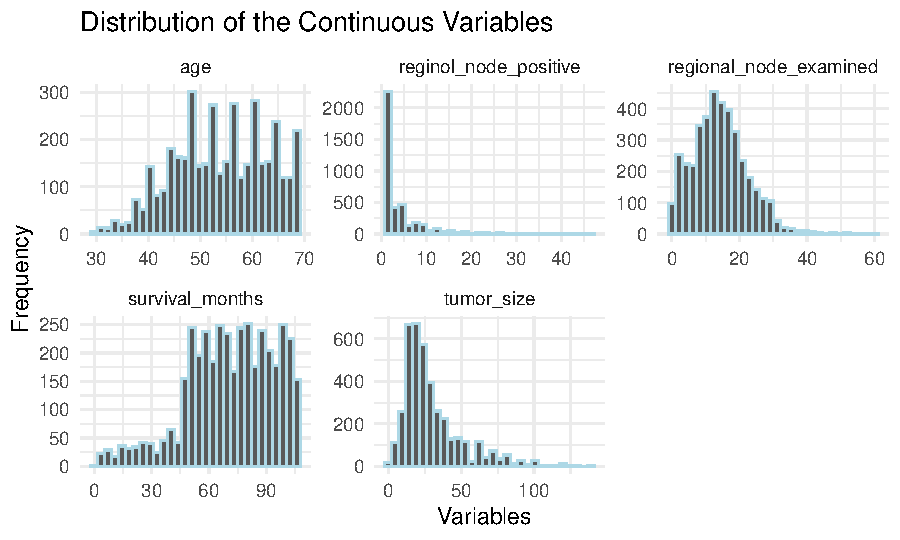
\includegraphics[width=0.9\linewidth]{P8130_project_report_files/figure-latex/distribution_of_the_continuous_variables-1} \caption{Distribution of the Continuous Variables}\label{fig:distribution_of_the_continuous_variables}
\end{figure}

\begin{figure}
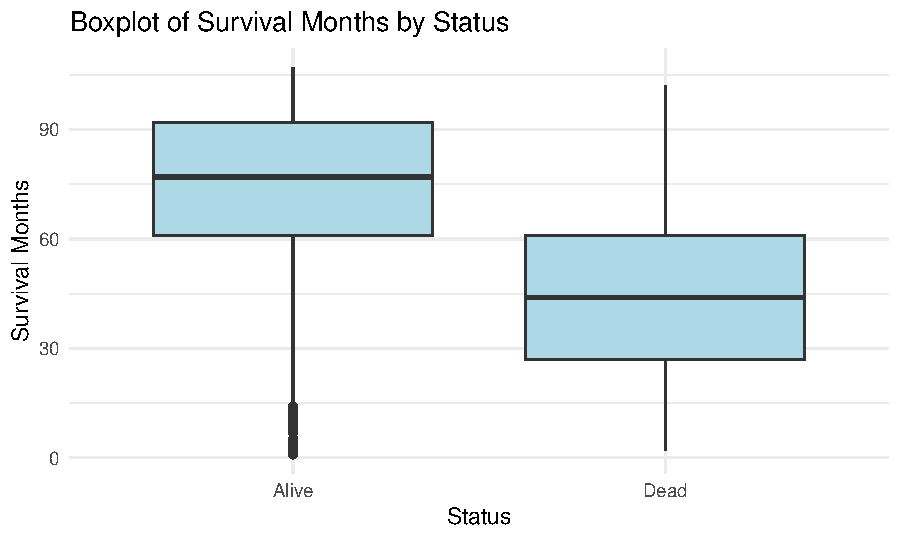
\includegraphics[width=0.9\linewidth]{P8130_project_report_files/figure-latex/survival_months_by_status-1} \caption{Survival Months by Status}\label{fig:survival_months_by_status}
\end{figure}

\begin{figure}
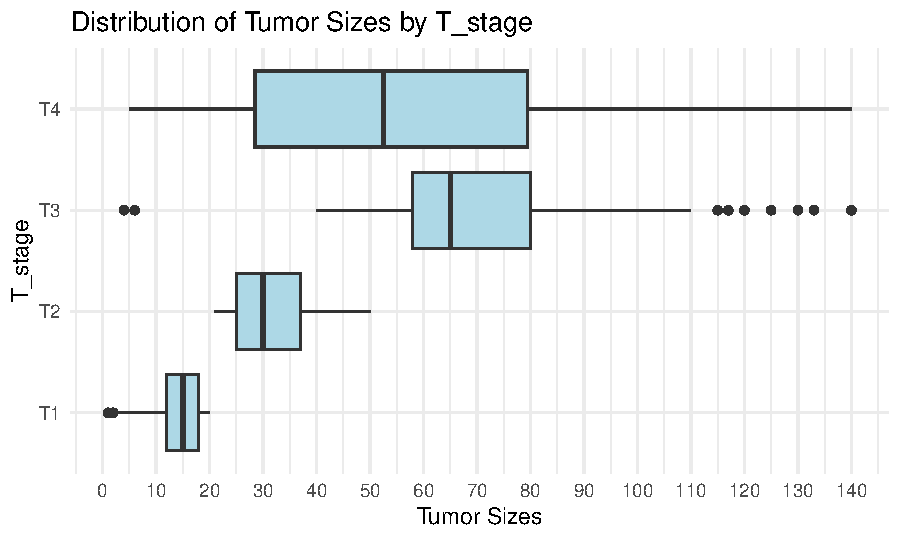
\includegraphics[width=0.9\linewidth]{P8130_project_report_files/figure-latex/tumor_sizes_by_t_stage-1} \caption{Tumor Sizes by T stage}\label{fig:tumor_sizes_by_t_stage}
\end{figure}

\begin{figure}
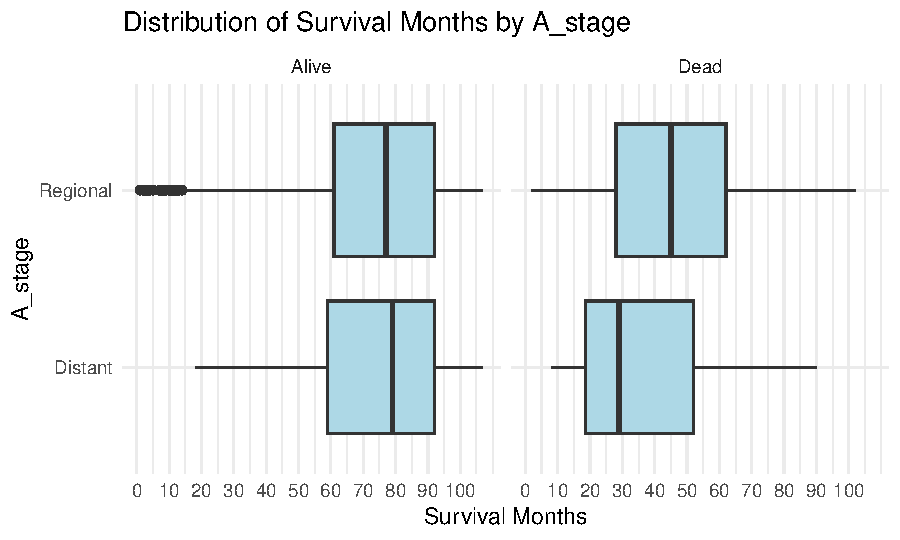
\includegraphics[width=0.9\linewidth]{P8130_project_report_files/figure-latex/survival_months_by_a_stage_based_on_status-1} \caption{Survival Months by A stage Based on Status}\label{fig:survival_months_by_a_stage_based_on_status}
\end{figure}

\begin{figure}
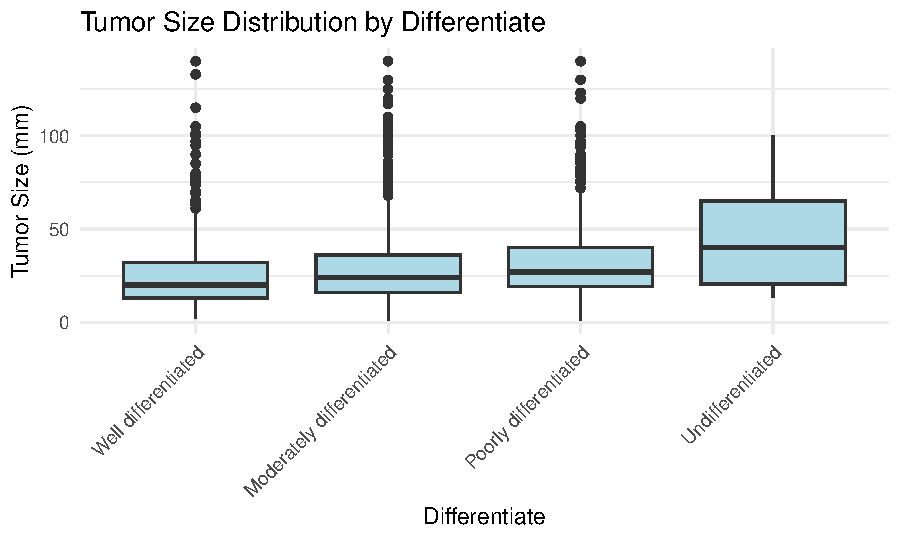
\includegraphics[width=0.9\linewidth]{P8130_project_report_files/figure-latex/tumor_size_by_differentiate-1} \caption{Tumor Size by Differentiate}\label{fig:tumor_size_by_differentiate}
\end{figure}

\begin{figure}
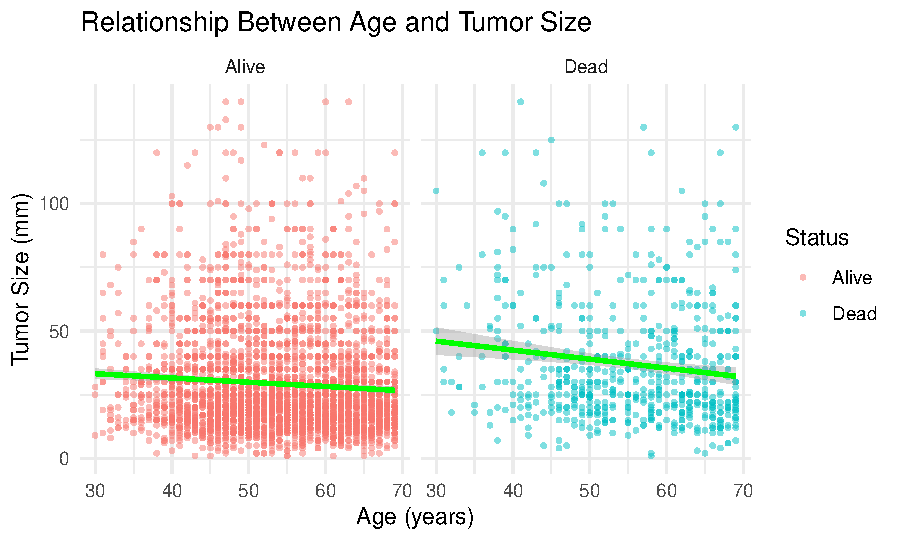
\includegraphics[width=0.9\linewidth]{P8130_project_report_files/figure-latex/relationship_between_age_and_tumor_size_across_status-1} \caption{Relationship Between Age and Tumor Size across Status}\label{fig:relationship_between_age_and_tumor_size_across_status}
\end{figure}

\begin{figure}
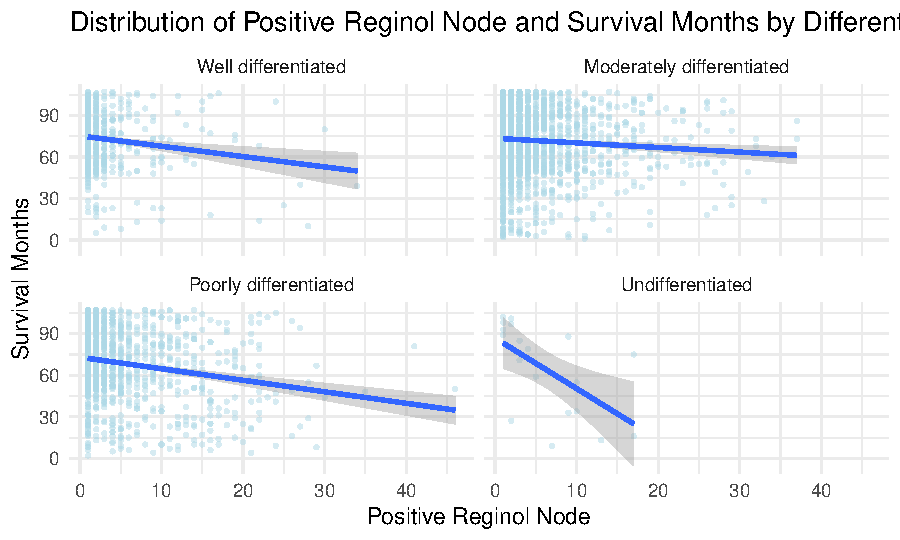
\includegraphics[width=0.9\linewidth]{P8130_project_report_files/figure-latex/positive_reginol_node_vs_survival_months_across_differentiate-1} \caption{Positive Reginol Node vs Survival Months Across Differentiate}\label{fig:positive_reginol_node_vs_survival_months_across_differentiate}
\end{figure}

\end{document}
